\section{ANITA sensitivity}
\label{sec:results}

The simulation files produced with \icemc are used by the ANITA analysts to tune analysis cuts, check the rate of accidental clustering, and also to simulate sources like Gamma Ray Bursts and Active Galactic Nuclei.
Finally, the simulation is used to calculate the experimental sensitivity.

\subsection{Acceptance}
\label{subsec:acceptance}
The ANITA collaboration uses \icemc to calculate the experiment volumetric acceptance \effvol, following:
\begin{equation}
  \label{eq:volacceptance}
  \effvol = \dfrac{n_{{pass}}(E)V_0\Omega}{N(E)} \;,
\end{equation}
\noindent where
 $n_{{pass}}(E)$ is the weighted (see Section~\ref{sec:weights}) number of events that pass the trigger at a given energy $E$,
 $V_0$ is the volume of ice in Antarctica viewed by ANITA,
$\Omega$ is $4\pi$ steradians, and 
 $N(E)$ is number of neutrinos thrown by each simulation at that energy $E$.

The ANITA acceptance (\effarea) is calculated following:
\begin{equation}
  \label{eq:acceptance}
  \effarea = \dfrac{\effvol}{\ell_{{int}}(E)} \;,
\end{equation}
\noindent where
 \effvol is the volumetric acceptance and
 $\ell_{{int}}(E)$ is the average interaction length in that energy bin. %\CD{I think we use the $\nu$ CC length, although we should do something a bit smarter than that. Do we want to be more specific here?} 
The interaction length is calculated following:
 \begin{equation}
   \label{eq:intlength}
    \ell_{{int}}(E_\nu) =   \dfrac{M_{NUCL}}{\sigma(E) \rho_{h_2o} } \;,
  \end{equation}
  
\noindent where
 $M_{NUCL}$ is the atomic nuclear mass ($1.66\cdot 10^{-27}$\,kg),
 $\rho_{h_2o}$ is the density of water (1000\,kg/m$^3$), 
and $\sigma(E)$ is the neutrino cross-section for $\nu$ charged-current interactions.
Currently the neutrino cross-section is calculated using either the
Reno {\it et al.}~\cite{reno2005high}
or the Connolly {\it et al.}~\cite{PhysRevD.83.113009} parametrizations.
The latter is the default.

Although recent neutrino cross-section measurements by the IceCube
Collaboration reached the multi-TeV
scale~\cite{aartsen2017measurement,bustamante2017measurement}, there
are still no measurements at energies above 10\,TeV.
The current theoretical models can extrapolate the cross-sections up to $10^{21}$\ev~\cite{PhysRevD.83.113009,reno2005high},
but the associated uncertainties are
large, and the impact on the ANITA acceptance is
non-negligible.
Figure~\ref{fig:acceptanceVSxsec}~(right) shows the effect of changing the
cross-section parametrization on the ANITA-III acceptance.
The nominal Connolly {\it et al.} parametrization is compared to the upper and lower bound set by
Reference~\cite{PhysRevD.83.113009}, and to the alternate
parametrization suggested by Reference~\cite{reno2005high}.


\begin{figure}[!h]\centering
  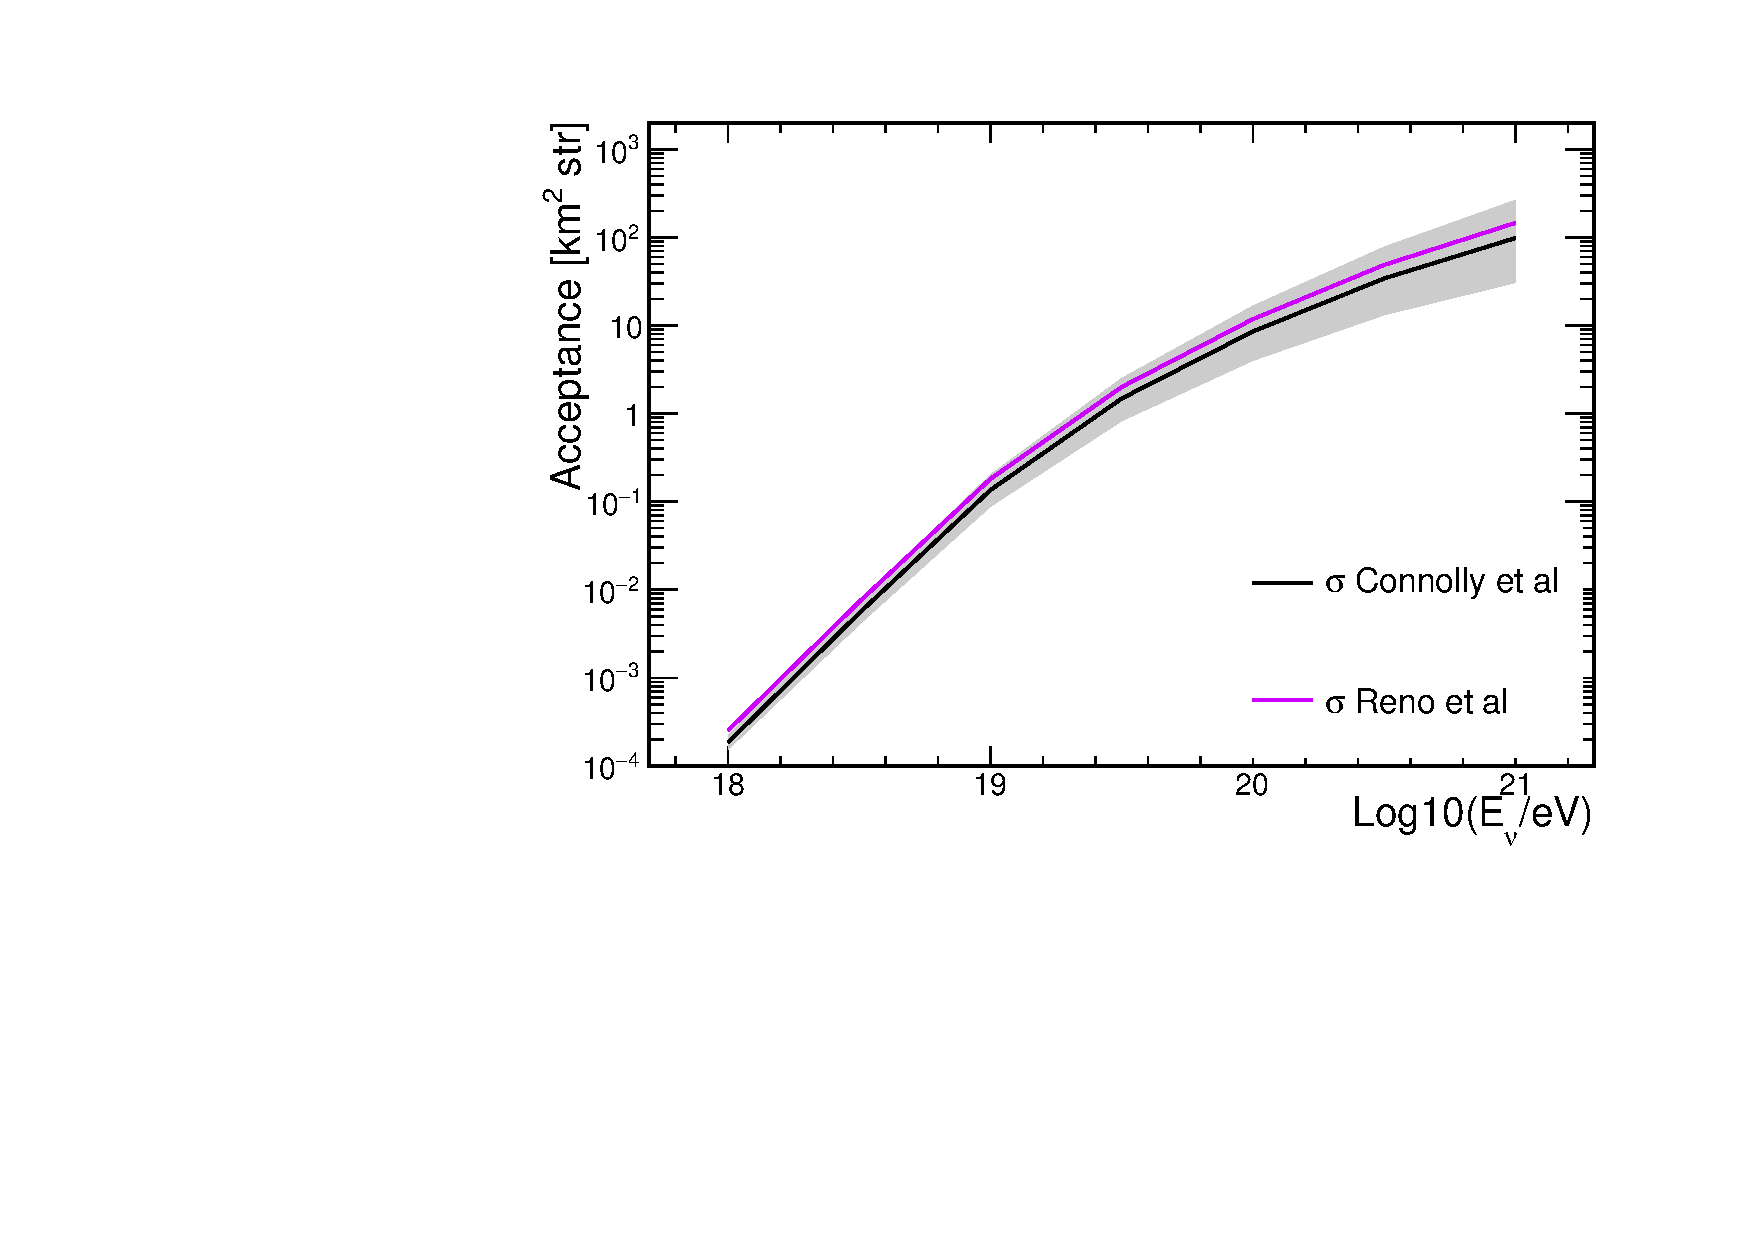
\includegraphics[width=.45\linewidth]{./Figs/AcceptanceVScrossSectionParam_ANITA3.pdf}
  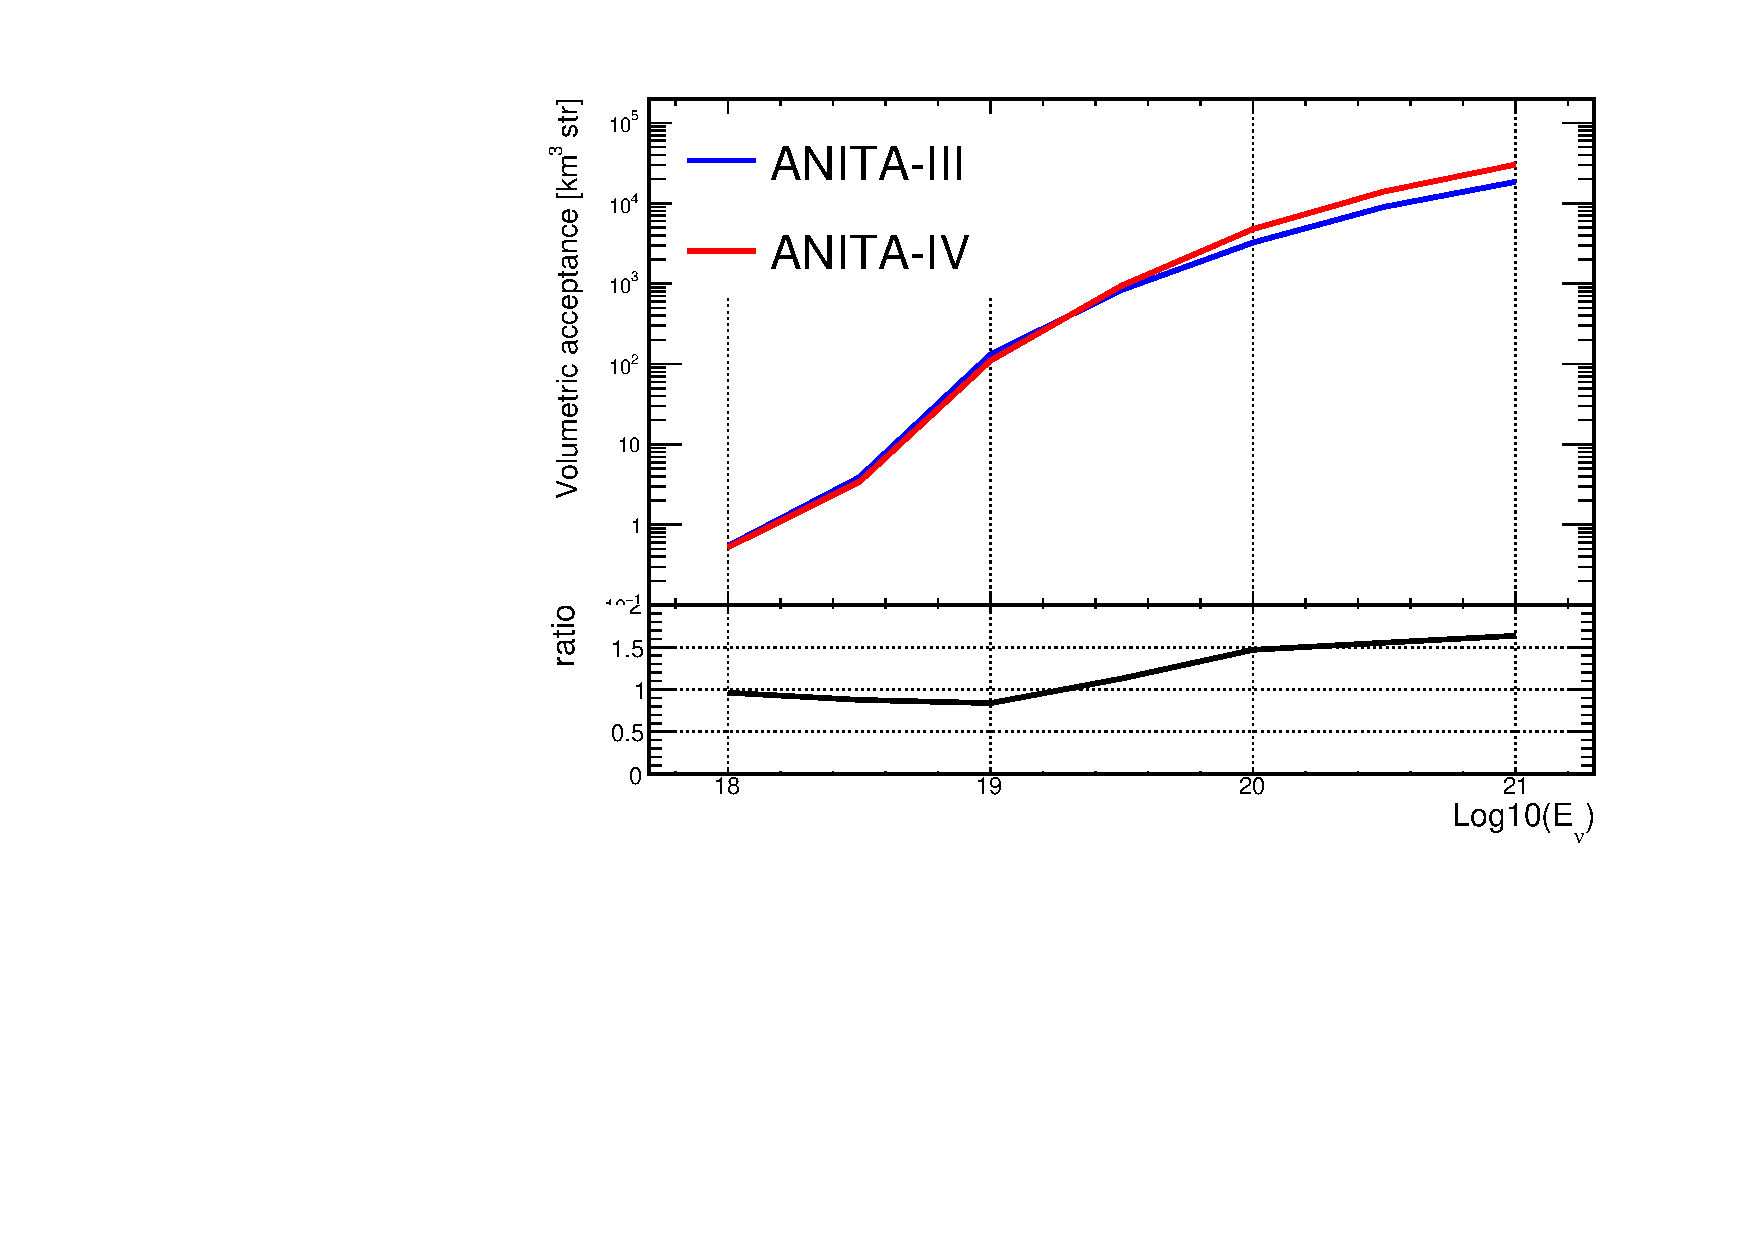
\includegraphics[width=.45\linewidth]{./Figs/CompareEffVol_A3vsA4.pdf}
  \caption{(Left) ANITA-III acceptance for different cross-section parametrizations: Connolly et al.~\cite{PhysRevD.83.113009} and Reno et al.~\cite{reno2005high}. (Right) ANITA-III and ANITA-IV volumetric acceptance comparison as a function of energy.}
  \label{fig:acceptanceVSxsec}
\end{figure}


\begin{figure}[!h]\centering
  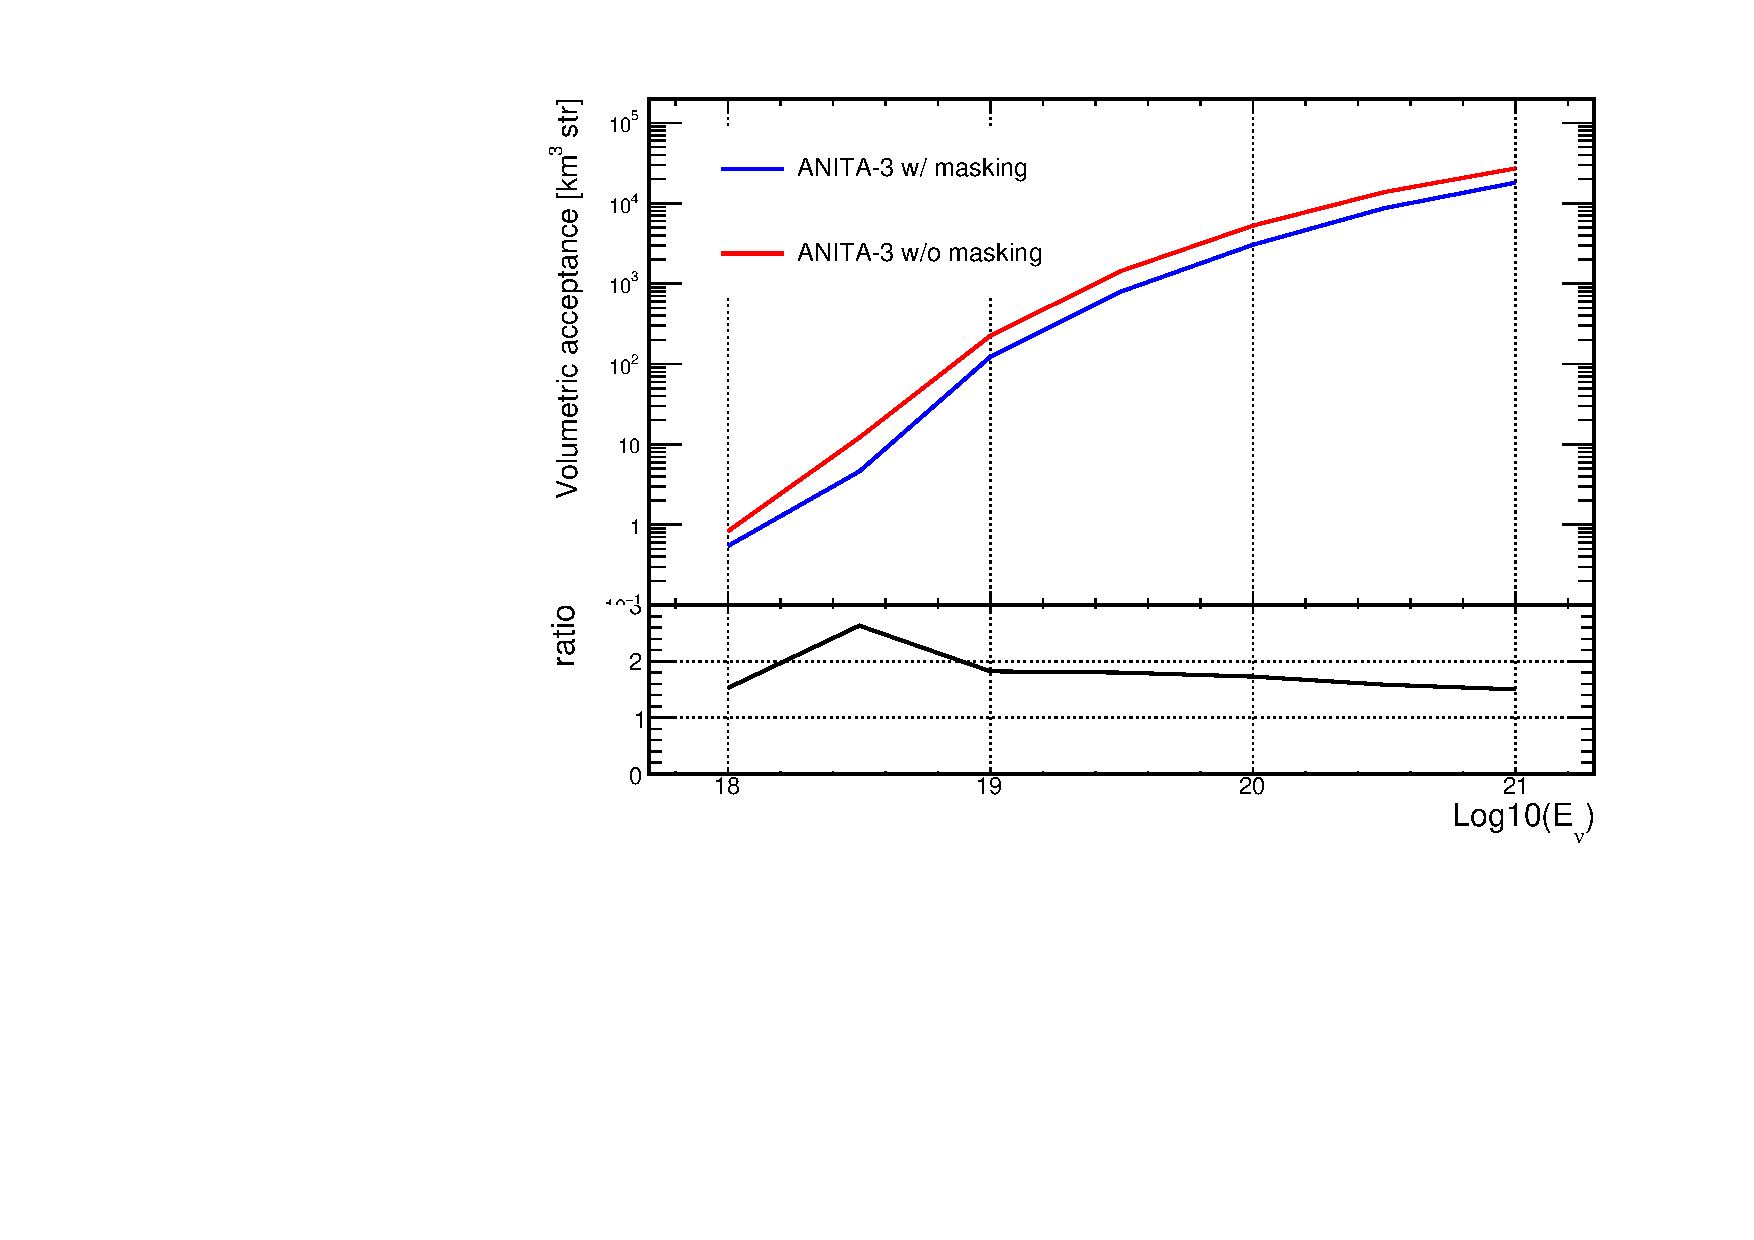
\includegraphics[width=.45\linewidth]{./Figs/CompareEffVol_A3masking.pdf}
  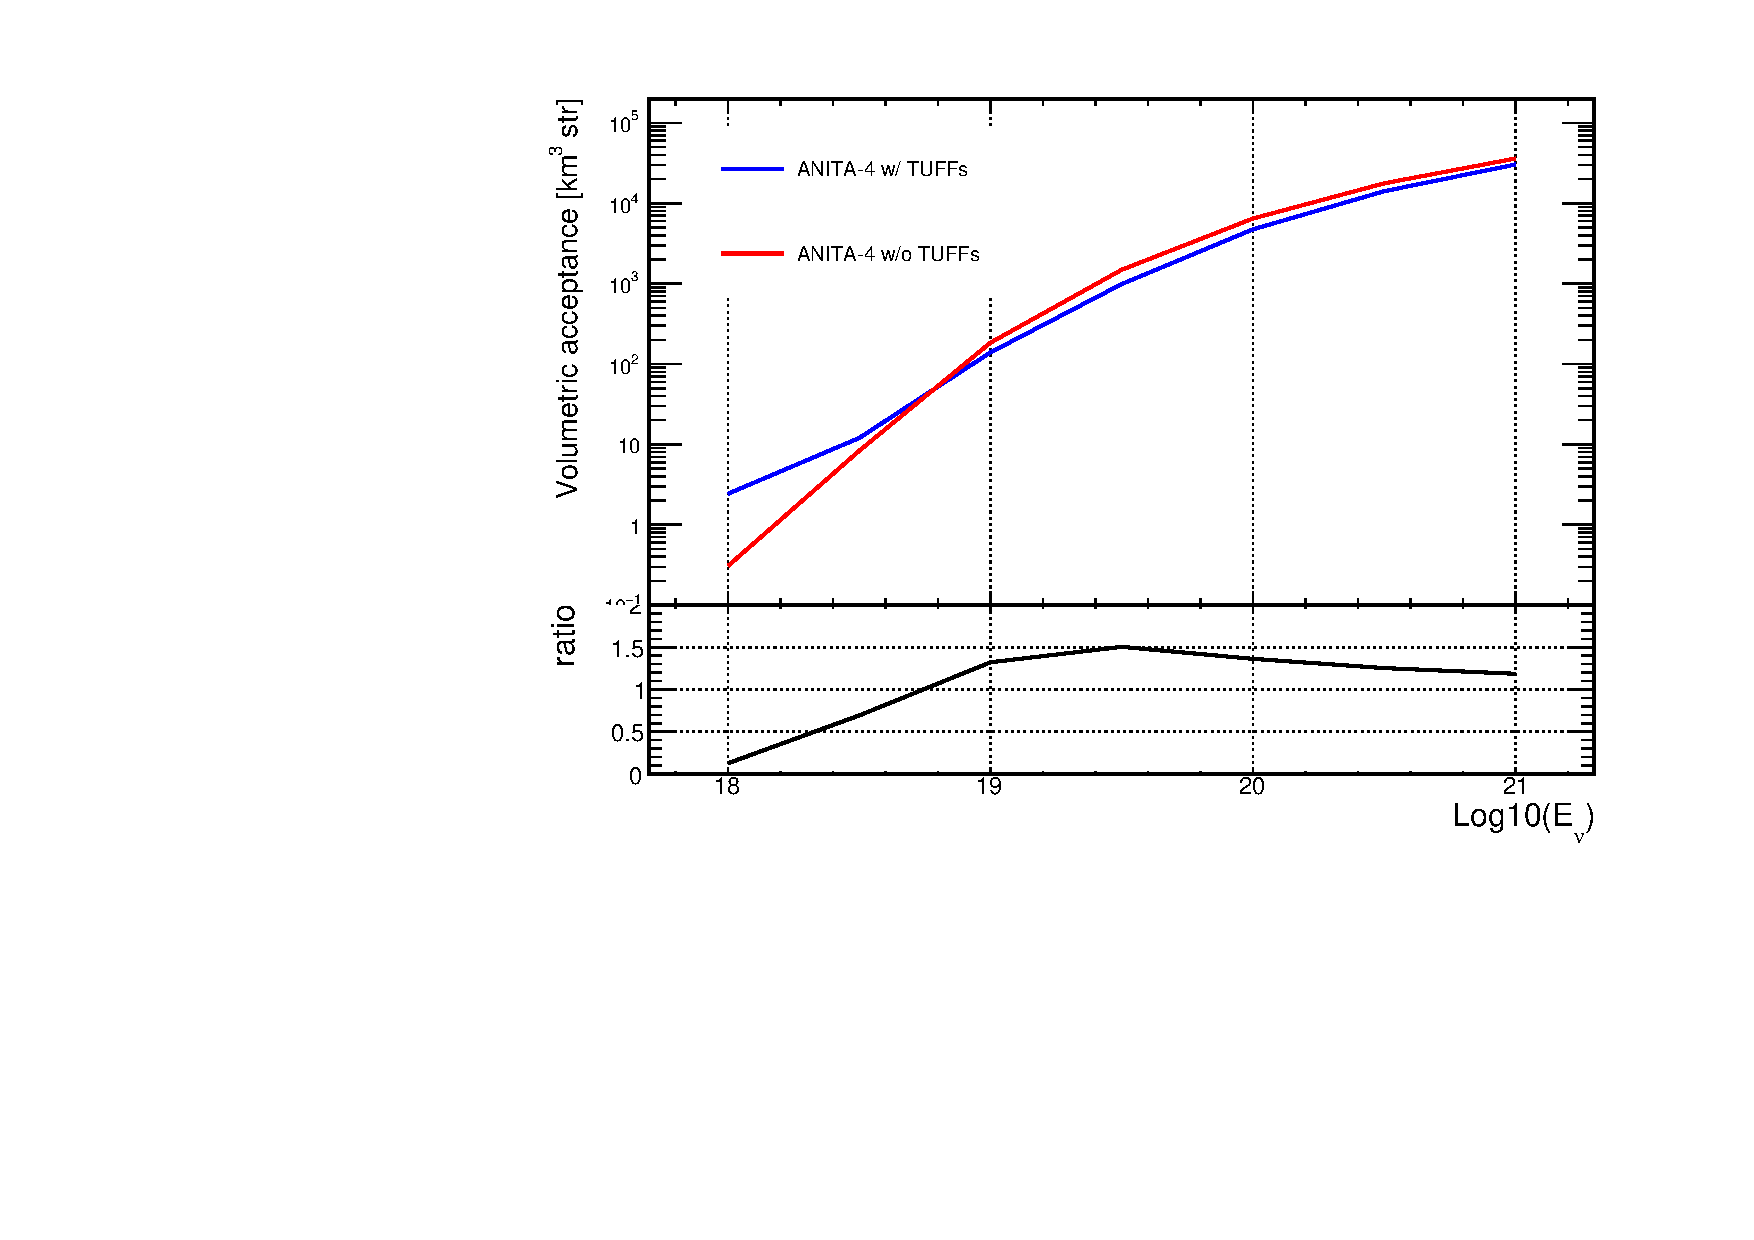
\includegraphics[width=.45\linewidth]{./Figs/CompareEffVol_A4tuff.pdf}
  \caption{(Left) Comparison of ANITA-III volumetric acceptance with and without channel masking.
  (Right) Comparison of ANITA-IV volumetric acceptance with and without TUFFs.}
  \label{fig:acceptanceVariations}
\end{figure}

Figure~\ref{fig:acceptanceVSxsec}(right) shows the ANITA-III and ANITA-IV volumetric acceptances and their ratio.
The ANITA-IV hardware improvements (use of better low noise amplifiers, the tunable notch filters to avoid carrier wave noise, and the use of LCP-RCP trigger coincidences to avoid satellite noise) enabled ANITA-IV to improve by 50\% at high energy.

Volumetric acceptances are also used to compare the impact of different hardware choices.
ANITA-III was highly affected by satellite noise and had to employ channel masking throughout the entire flight to avoid overloading the trigger. Figure~\ref{fig:acceptanceVariations}~(left) shows that channel masking reduced the ANITA-III sensitivity by more than 50\% across all energy bins.
ANITA-IV used the TUFF boards to avoid carrier wave noise: Figure~\ref{fig:acceptanceVariations}~(right) shows the impact of the tunable filters on the ANITA-IV sensitivity which was reduced by 25--50\%.

Figure~\ref{fig:moreAcceptanceVariations} shows the variation of the ANITA-IV volumetric acceptances coming from different \icemc parameter variations.
The black solid line shows the effect of using BEDMAP instead of CRUST 2.0 as Antarctica ice model; the more finely binned BEDMAP map results in a roughly 20\% lower acceptance over all energies.
The orange solid lines shows the effect of varying the random surface inclination, the two cases shows are 0 and 2.4\%, where the latter is double the nominal value.
The violet area shows the effect of using constant trigger thresholds instead of time varying thresholds; the dashed violet area is the result of using the minimum and maximum thresholds for the whole flight.

\begin{figure}[!h]\centering
  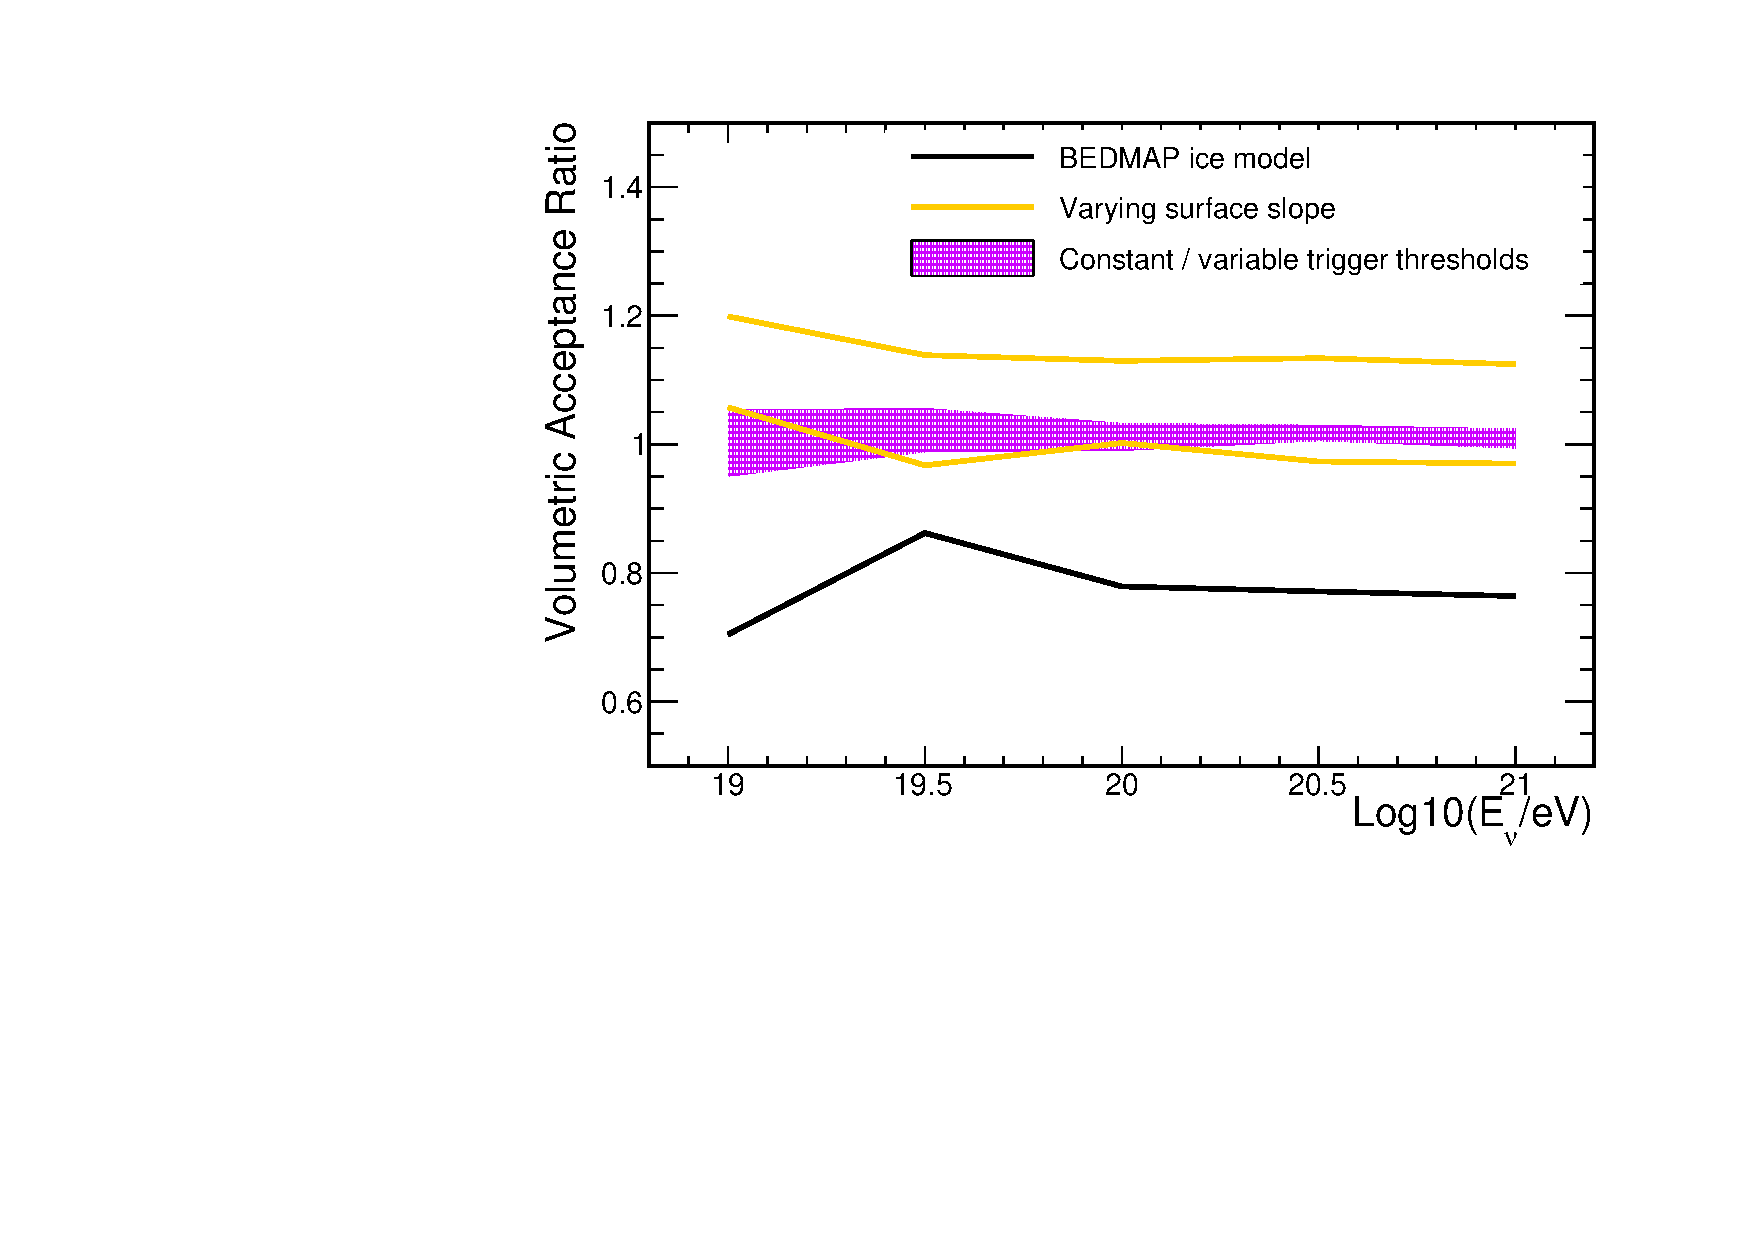
\includegraphics[width=.45\linewidth]{./Figs/SystUncertaintiesForPaper.pdf}
  \caption{Ratio of ANITA-IV volumetric acceptances as a function of energy found varying different \icemc parameters. The solid black line shows the variation coming from using BEDMAP instead of CRUST 2.0 as Antarctica ice model.
  The orange solid lines are calculated by setting the surface slope inclination at 0 or 2.4\% (double the nominal).
  The violet dotted area is found by using constant trigger thresholds instead of time varying thresholds. }
  \label{fig:moreAcceptanceVariations}
\end{figure}

\subsection{Limit}
\label{subsec:limit}
The projected 90\% confidence level on the diffuse neutrino flux is set by using:
\begin{equation}
\left( \dfrac{Ed^4N}{dE dA d\Omega dt}\right)_{lim} =
\dfrac{s_{up}}{ T \cdot \epsilon_{ana} (E_\nu) \cdot \effarea \cdot \Delta} \, ,
\end{equation}
\noindent
where
$s_{up}$ is the upper (one-sided) limit for the mean of a Poisson
variable given 0 observed events in the absence of background for 90\%
CL, 
$T$ is the live time 
(17.4 days for ANITA-III and 24.25 days for ANITA-IV), 
$\epsilon_{ana}(E_\nu)$ is the neutrino analysis efficiency,
\effarea is the experiment acceptance as a function of the neutrino
energy, and $\Delta=4$ is a model-independent factor following Reference~\cite{PhysRevD.73.082002}.


Figure~\ref{fig:sensitivity} shows the ANITA-III, ANITA-IV and ANITA\,I-IV limits as calculated in References~\cite{anita3cosmogenic,anita4cosmogenic}.
These are compared to the latest constraints coming from the IceCube~\cite{icecube2018} and Auger experiments~\cite{auger2017}, as well as
four cosmogenic neutrino models~\cite{kkss2002,takami2009,ahlers2012,kotera2010cosmogenic}.

\begin{figure}[!h]\centering
 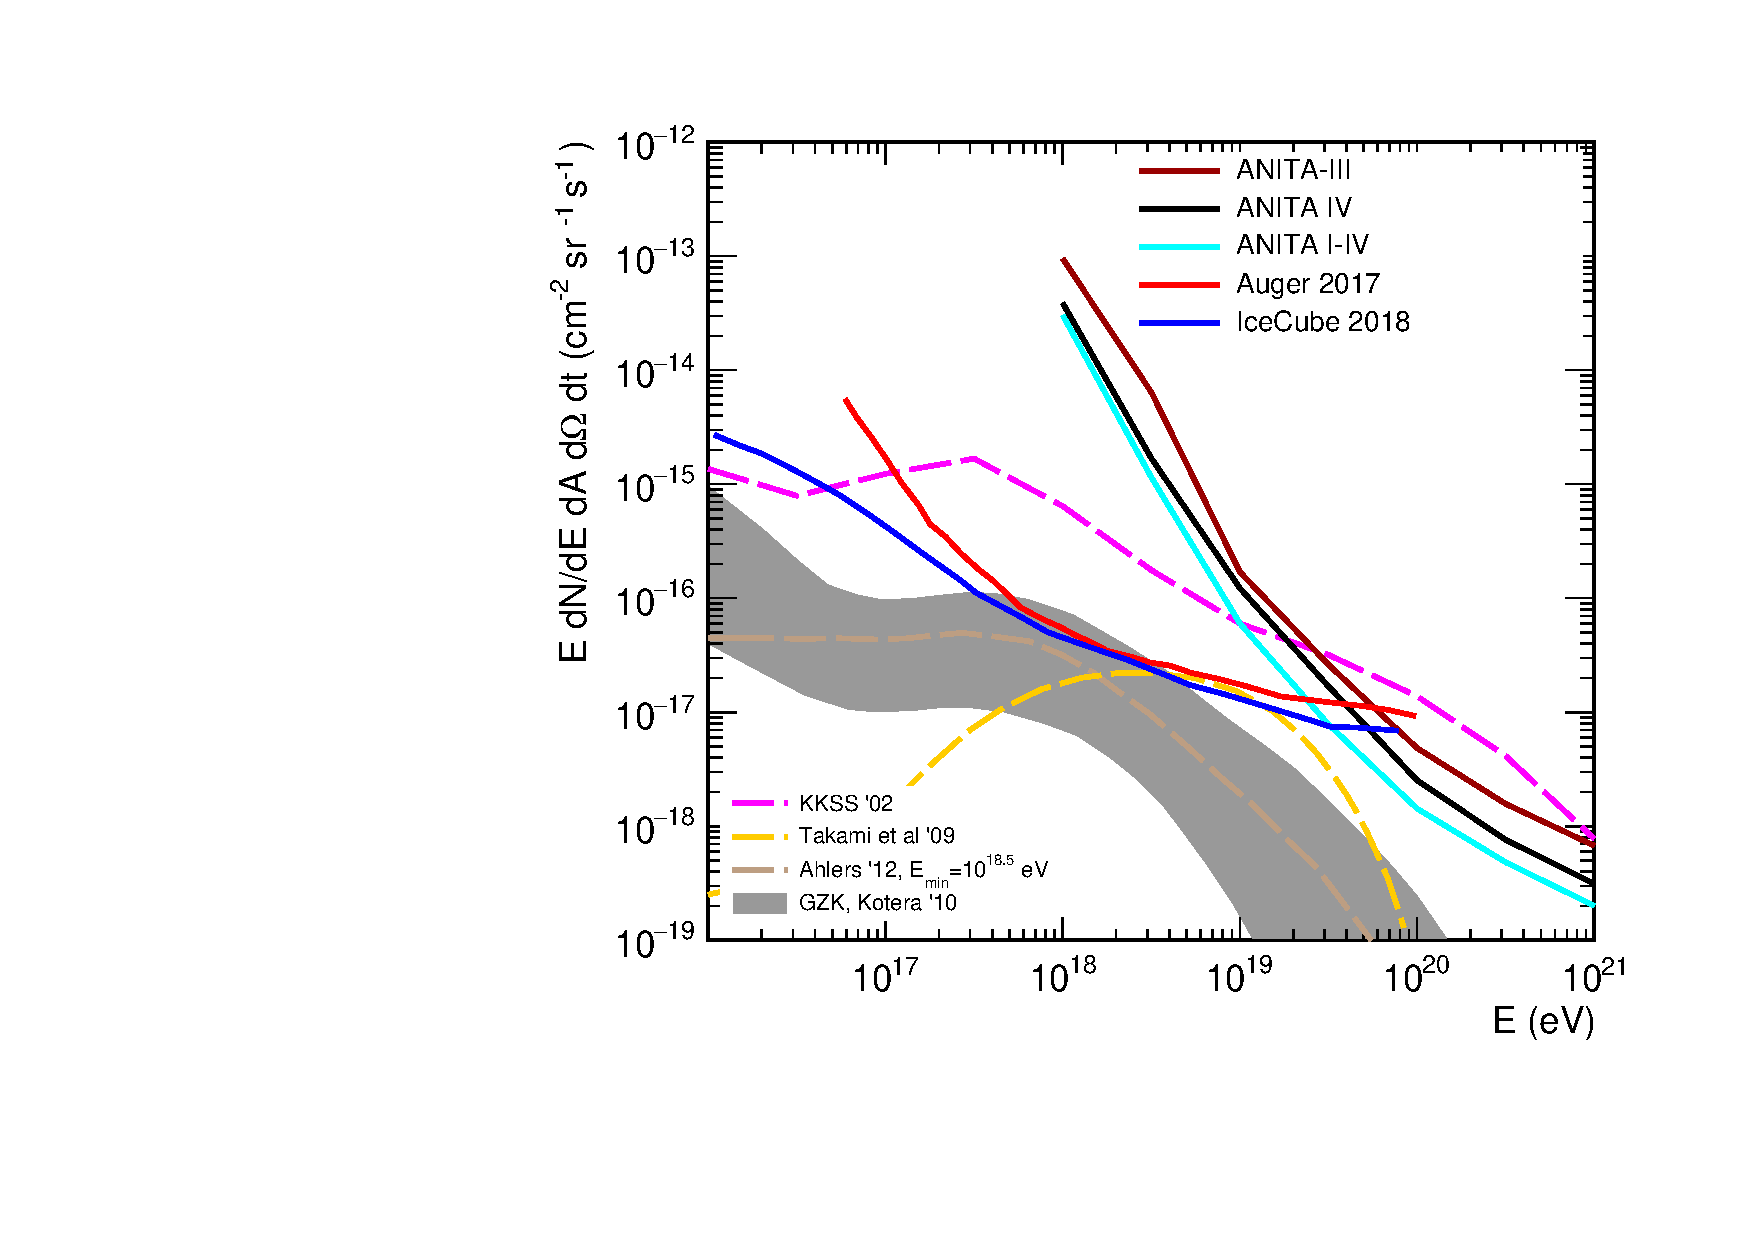
\includegraphics[width=.65\linewidth]{./Figs/Limit4icemcPaper.pdf}
 \caption{
 ANITA-III and ANITA-IV limit on the all flavor diffuse UHE neutrino flux and a combined limit from ANITA I-IV, as calculated in References~\cite{anita3cosmogenic,anita4cosmogenic}.
 The most recent UHE neutrino limits
from the Auger~\cite{auger2017} and IceCube~\cite{icecube2018} experiments, and
four cosmogenic neutrino models~\cite{kkss2002,takami2009,ahlers2012,kotera2010cosmogenic} are also displayed. 
}
 \label{fig:sensitivity}
\end{figure}

%\subsection{Expected number of events}
%\label{subsec:events}
%Using the acceptance, \effarea, and the fluence, EF(E), relative to a
%specific flux model, the expected number of events
%detected by the ANITA-III flight, is calculated as follows:
%\begin{equation}
%  n_{obs} = \log(10) \int dT \int d\log_{10} (E/\ev)
%  \effarea EF(E) \, ,
%\label{eq:numobs}
%\end{equation} 
%\noindent where $T$ is the experiment live time.
%
%Table~\ref{tab:nobs} shows the expected numbers of events observed by
%ANITA-III from several cosmogenic neutrino models.
%
%The Ave et al fluxes~\cite{ave2005cosmogenic} consider proton or iron primaries.
%For iron primaries, the expected neutrino flux highly depends on the cosmological evolution, $n$,
%of the source, and on the maximum cosmic ray energy at the source, $E_{max}$.
%The Kotera et al fluxes~\cite{kotera2010cosmogenic} use a  mixed chemical composition model for which the extragalactic cosmic
%ray composition at the source is assumed to be similar to that of low energy Galactic cosmic rays.

%\subsection{Parameter variations} 
%label{subsec:uncertainties}
%In this Subsection we explore how varying some of the physics model
%parameters affects the projected ANITA sensitivity.
%%Can run some test simulations to study these 

%\subsubsection{Varying cross-section models}
%\label{subsubsec:uncertainties_xsec}

%\subsubsection{Varying thresholds}
%\label{subsubsec:uncertainties_threshold}


%\subsubsection{Varying ice thickness models}
%\label{subsubsec:uncertainties_ice}
%\todo[inline]{LINDA: calculate acceptance changes with different ice thicknesses of CRUST 2.0}


\section{Summary and Future improvements}
\label{sec:future}
The \icemc Monte Carlo simulation tool is used for the
simulation of ultra high energy neutrino interactions in the Antarctic
ice and their detection by the ANITA experiment.
The data taken before or during the ANITA flights are used to validate the
simulation.
The latest ANITA-III, ANITA-IV and ANITA\,I-IV performance is provided in the form of the
acceptance and energy dependent neutrino limit.
 
Future versions of the tool will include the possibility to use extensive air showers inputs from ZHAireS~\cite{alvarez2012monte}; improved and refined ice properties modeling and surface roughness effects; the contribution of the sun to the thermal noise; and carrier wave noise as measured during the ANITA-III and ANITA-IV flights.
We are also working towards expanding the framework so that it can be used by all radio experiments based in Antarctica.
